
\chapquote{``In the mind's eye, a fractal is a way of seeing infinity."}{James Gleick}

\problem The \textit{Sierpinski Carpet} is a plane fractal. It can be produced iteratively by taking a solid square, dividing
it into 9 congruent squares in a 3-by-3 grid, removing the centre square, and recursively applying the same procedure on each
of the remaining squares \textit{ad infinitum}.

Display the \textit{Sierpinski Carpet} to a specified number of iterations. 

\begin{figure}[h]
	\begin{center}
		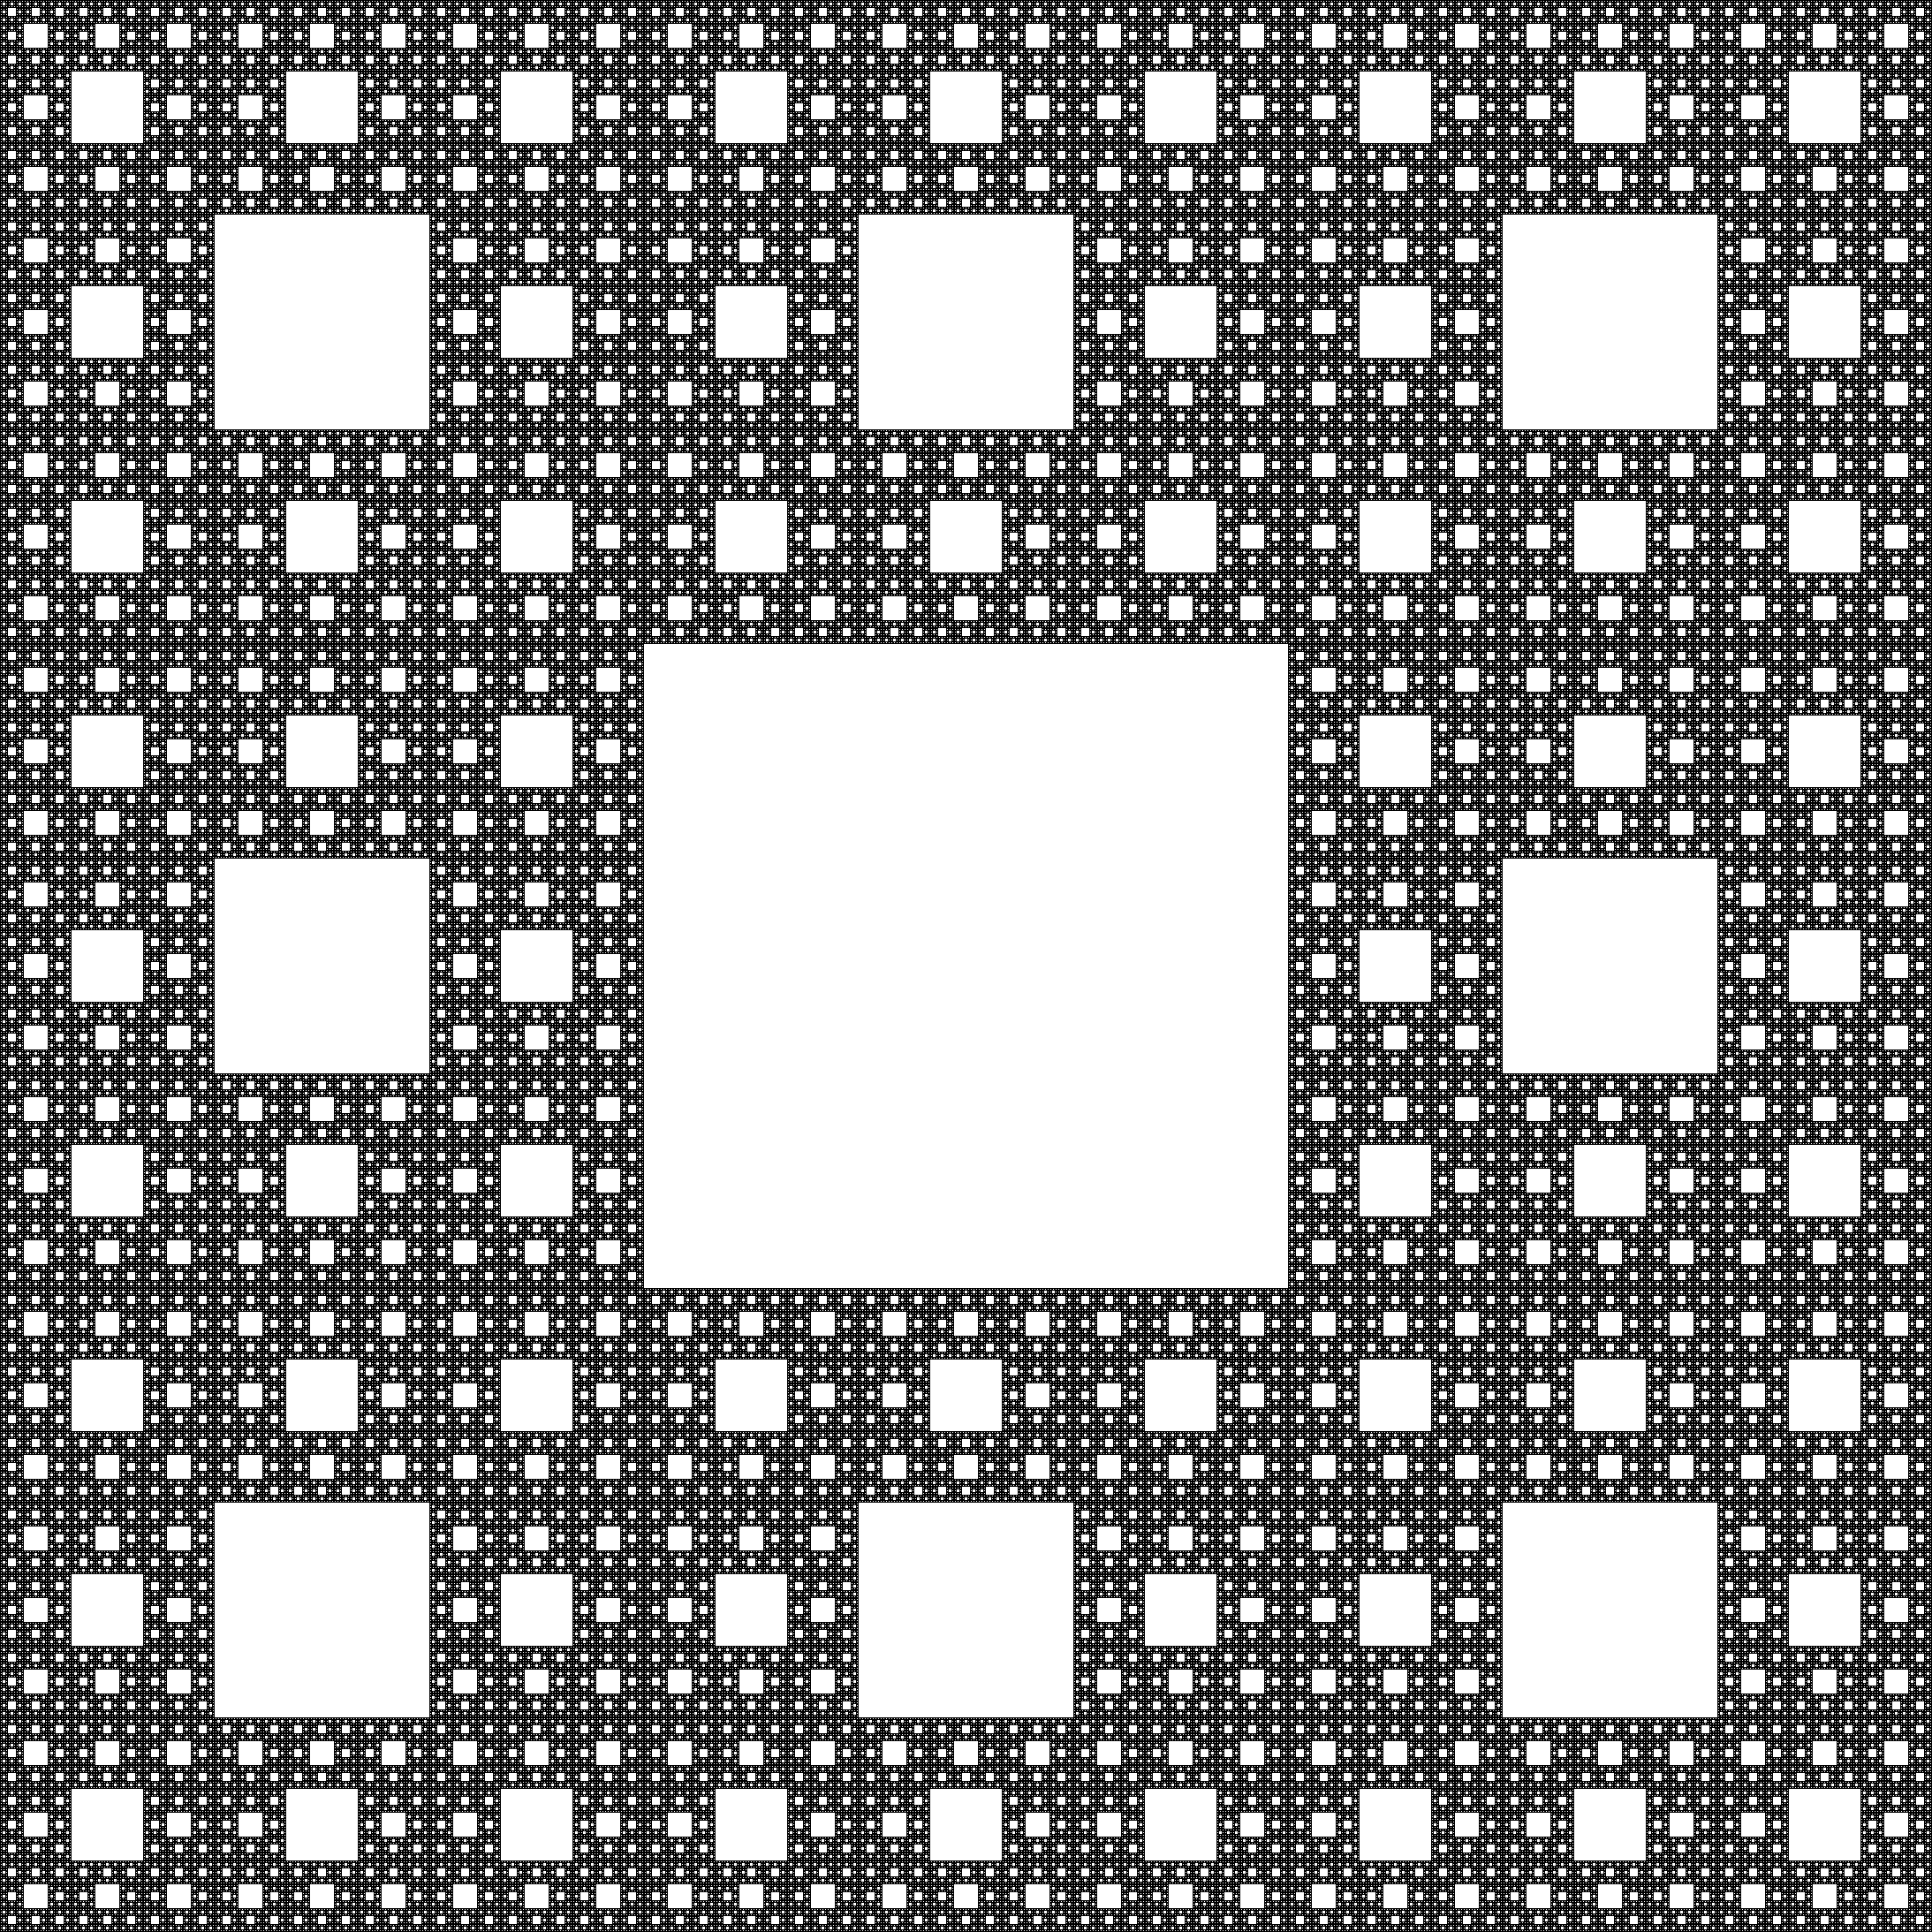
\includegraphics[scale=0.15]{sierpinski.png}
	\end{center}
	\caption*{The Sierpinski Carpet}
	\label{fig:sierpinski_carpet}
\end{figure}

\solution In an ASCII terminal, we can only display a rough representation of the \textit{Sierpinski Carpet}, a few levels deep.
A level $n$ carpet will have a width and height of $3^n$. Within this grid, every character lies either in the centre of a 3-by-3
square, in which case it is not in the carpet, or it lies on the edge, in which case it is in the carpet. If neither can be 
determined, we can scale up the search square to the next level, and repeat recursively.

Here, points in the carpet are drawn, while points not in the the carpet are left as whitespace.

\algorithm
\texttt{main (level:Integer)}
\begin{enumerate}
	\item For each pair (\texttt{i} , \texttt{j}) $\in \{0, 1, \dots, 3^n - 1\} \times \{0, 1, \dots, 3^n - 1\}$:
	\begin{enumerate}
		\item Call \texttt{isInSierpinskiCarpet(i, j)}. If it returns \texttt{true}, display a solid block
			at (\texttt{i}, \texttt{j}), otherwise, leave a blank space there.
	\end{enumerate}
	\item \textbf{Exit} 
\end{enumerate}
\vspace{5mm}
\texttt{isInSierpinskiCarpet (x:Integer, y:Integer)}
\begin{enumerate}
	\item If either of \texttt{x} or \texttt{y} is zero, the point (\texttt{x}, \texttt{y}) is on the edge of
		a square of some level. \textbf{Return} \texttt{true}.
	\item If both \texttt{x} and \texttt{y} leave a remainder of one on division by $3$, the point (\texttt{x}, \texttt{y})
		is at the centre of a square of some level. \textbf{Return} \texttt{false}.
	\item Call \texttt{isInSierpinskiCarpet(x / 3, y / 3)}, and \textbf{return} the returned value.
\end{enumerate}

\sourcecode
\lstinputlisting{src/SierpinskiCarpet.java}

\varDescription
\begin{longtable} {| >{\ttfamily}p{0.16\linewidth} | >{\ttfamily}p{0.2\linewidth}| p{0.6\linewidth} |}
\hline\multicolumn{3}{|c|}{\tt SierpinskiCarpet::main(String[])} 		\\\hline
int 		&	level		&	The depth to which to render the carpet \\\hline
int 		&	i, j		&	Counter variables, represent a point on the screen to be displayed \\\hline
\hline\multicolumn{3}{|c|}{\tt SierpinskiCarpet::isInSierpinskiCarpet(int, int)} 		\\\hline
int 		&	x, y		&	Counter variables, represent the point in question \\\hline
\end{longtable}
